\documentclass{article}

\usepackage{graphicx}
\usepackage{arxiv}
\graphicspath{ {images/} }
\usepackage[utf8]{inputenc} % allow utf-8 input
\usepackage[T1]{fontenc}    % use 8-bit T1 fonts
\usepackage{hyperref}       % hyperlinks
\usepackage{url}            % simple URL typesetting
\usepackage{booktabs}       % professional-quality tables
\usepackage{amsfonts}       % blackboard math symbols
\usepackage{nicefrac}       % compact symbols for 1/2, etc.
\usepackage{microtype}      % microtypography
\usepackage{lipsum}


\title{a study in GANs}
\author{
   Aniket Das (Mentor)\\
   Department of Electrical Engg.\\
   IIT Kanpur\\
   \texttt{aniketd@iitk.ac.in} \\
   \And
    Avik Pal(Mentor)\\
     Department of Computer Science and Engg.\\
     IIT Kanpur\\
     \texttt{avikpal@iitk.ac.in}\\
     \And
     Naman Biyani\\
     Department of Computer Science and Engg.\\
     IIT Kanpur\\
     \texttt{namanb@iitk.ac.in} \\
     \And
     Nirmal Suthar\\
     Department of Computer Science and Engg.\\
     IIT Kanpur\\
     \texttt{nirmalps@iitk.ac.in} \\
     }
   %% \AND
   %% Coauthor \\
%   %% Affiliation \\
%   %% Address \\
%   %% \texttt{email} \\
%   %% \And
%   %% Coauthor \\
%   %% Affiliation \\
%   %% Address \\
%   %% \texttt{email} \\
%   %% \And
%   %% Coauthor \\
%   %% Affiliation \\
%   %% Address \\
%   %% \texttt{email} \\
% }


\begin{document}
\maketitle
% keywords can be removed
%\keywords{First keyword \and Second keyword \and More}
\begin{center}
    {\Large{\textbf{Introduction}}}
\end{center}

Image synthesis is an important problem in computer vision. There has been remarkable progress in this direction with the emergence of Generative Adversarial Networks (GANs). GANs have
been known to be unstable to train, often resulting in generators that produce nonsensical outputs/images (Figure 1). However GANs based on deep convolutional networks have been successful and especially in image generation in computer vision with the help of convolution which opens the possibility to explore multilayer GANs (DCGAN). In an unconditioned generative model, there is no control on modes of the data being generated.
However, by conditioning the generator on additional information (such as classes or label) it is possible to generate more specific. Such conditioning could be based on class labels (CGAN).

However, one can observe that convolutional GANs have mush more difficulty in modeling some image classes . For example, while the state-of-the-art GANs model excels at synthesizing image classes which are distinguished more by texture than by geometric or structural patterns that occur consistently in some classes. One possible explanation for this is that GANs models rely heavily on convolution to model the  dependencies across different image regions. Since the convolution operator has a local receptive field, long range dependencies can only be processed after passing through several convolutional layers. This could prevent learning about long-term dependencies for a variety of reasons. So adding self-attention mechanism into the convolutional GANs helps with modeling long-range dependencies (SAGAN).

\begin{figure}[h]
    \centering
    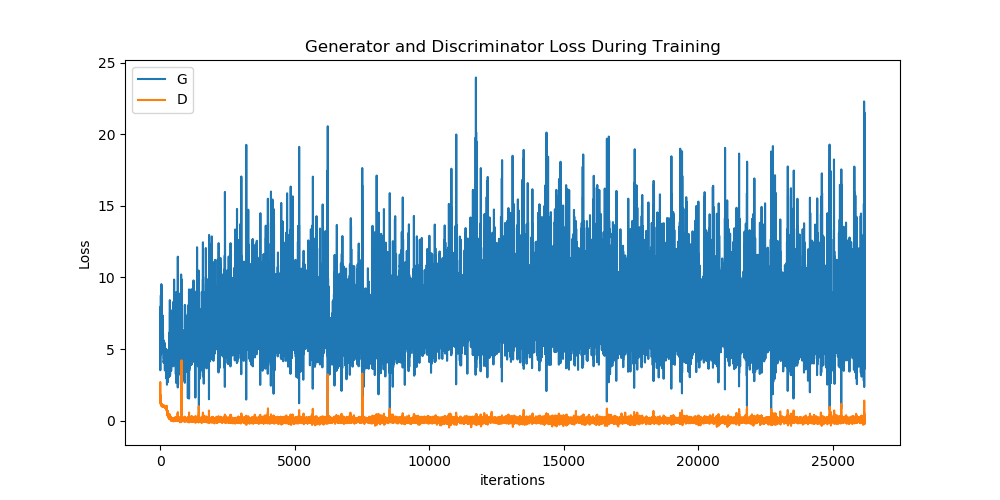
\includegraphics[width=.8\textwidth]{images/intro_progress.png}
    \caption{Loss of generator and discriminator during training DCGAN on MNIST dataset suggest that the GANs are unstable and special techniques should be used to train GANs effectively}
    \label{fig:mesh1}
\end{figure}
\medskip


\medskip
\begin{center}
    {\Large{\textbf{Related Work}}}
\end{center}
Until recently, most work on deep generative models focused on models that provided a parametric
specification of a probability distribution function. The model can then be trained by maximiz-
ing the log likelihood. In this family of model, perhaps the most succesful is the deep Boltzmann
machine . Such models generally have intractable likelihood functions and therefore require
numerous approximations to the likelihood gradient .

Unlike generative adversarial networks, variational autoencoders (VAE) pair a differentiable
generator network with a second neural network. Unlike generative adversarial networks, the sec-
ond network in a VAE is a recognition model that performs approximate inference. GANs require
differentiation through the visible units, and thus cannot model discrete data, while VAEs require
differentiation through the hidden units, and thus cannot have discrete latent variables. Other VAE-
like approaches exist but are less closely related to our method.
\medskip


\begin{center}
    {\Large{\textbf{Working of GANs}}}
\end{center}
We define a generator which input a noise and outputs a desired result which fools the discriminator, supposed to distinguished the generator output. To learn the generator’s distribution p\textsubscript{g} over data \textbf{\textit{x}}, we define a prior on input noise variables p\textsubscript{z}(\textbf{\textit{z}}), then represent a mapping to data space as G(\textbf{\textit{z}}; $\theta$\textsubscript{g}), where G is a differentiable function represented by a multilayer perceptron with parameters $\theta$g. We also define a
second multilayer perceptron D(\textbf{\textit{x}}; $\theta$\textsubscript{d}) that outputs a single scalar. D(\textbf{\textit{x}}) represents the probability
that x came from the data rather than p\textsubscript{g}. We train D to maximize the probability of assigning the
correct label to both training examples and samples from G. We simultaneously train G to minimize
log(1 - D(G(\textbf{\textit{z}}))) (Figure 2):


Finally, $\mathcal{L}_{GAN}$ is the generative adversarial network cost. That cost function represents the \textit{game} between $G$ and $D$.
When training $D$, $G$ are kept fixed and we have: 

\begin{figure}[h]
    \centering
    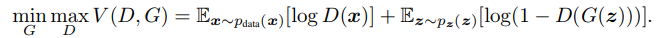
\includegraphics[width=.7\textwidth]{images/gan_equation.png}
    \caption{In other words, D and G play the following two-player minimax game with
value function V (G, D)}
    \label{fig:mesh1}
\end{figure}

For better gradient behavior of generator loss we minimize
\begin{equation}
 \mathcal{L}_{GAN}^{G} =  - log(D(G(z)))
\end{equation}

instead of
\begin{equation}
 \mathcal{L}_{GAN}^{G} =  log[1 - D(G(z))]
\end{equation}

\begin{figure}[h]
    \centering
    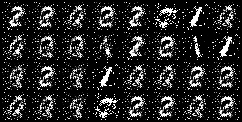
\includegraphics[width=.6\textwidth]{images/basicgan_result.png}
    \caption{Hand-digit generation tranined on MNIST dataset train by basicGAN}
    \label{fig:mesh1}
\end{figure}



\medskip
\begin{center}
    {\Large{\textbf{Deep Convolutional GANs}}}
\end{center}
It is worth thinking about the DCGAN as a foundational pillar for GANs research (Figure 4). The DCGAN model’s fundamental component is to replace the fully connected layers in the generator with these upsampling convolutional layers. In designing this architecture, the authors cite three sources of inspiration.

\begin{itemize}

    \item The All Convolutional Net → Replacing pooling operations with spatial downsampling convolutions
    \item Eliminating fully connected layers after convolutions
    \item Batch Normalization → Normalizing activations to help gradient flow

\end{itemize}

With these advancements in mind, the authors searched for a stable DC-GAN architecture and landed on the following architectural guidelines:

\begin{itemize}

    \item Replace any pooling layers with strided convolutions in the discriminator and fractional-strided convolutions in the generator
    \item Use Batch Normalization in the generator and discriminator
    \item Remove fully connected hidden layers for deeper architectures
    \item Use ReLU activation in generator for all layers except for Tanh in output (These images are normalized between [-1, 1] rather than [0,1] , thus Tanh over sigmoid)
    \item Use LeakyReLU activation in the discriminator for all layers

\end{itemize}


\begin{figure}[h]
    \centering
    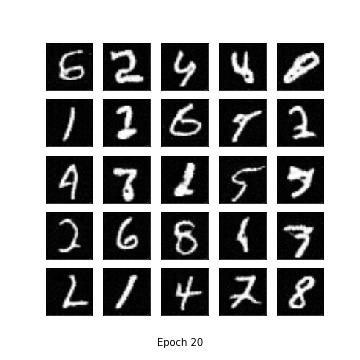
\includegraphics[width=.5\textwidth]{images/dcgan_result.png}
    \caption{Hand-generated digits generated on MNIST dataset train by DCGAN is huge improvement over digits generated by original GAN paper, suggest that use of convolution operation can be beneficial in GAN. }
    \label{fig:mesh1}
\end{figure}
\medskip


\medskip

\medskip
\begin{center}
    {\Large{\textbf{Class Conditioned GANs}}}
\end{center}
Class conditioned GANs proposes a simple extention of GANs that employs label conditioning in additional to produce high resolution and high quality generated images.

By adding an auxiliary classifier to the discriminator of a GANs, the discriminator produces not only a probability distribution over sources but also probability distribution over the class labels. This simple modification to the standard DCGAN models does not give tremendous difference but produces better results and is capable of stabilizing the whole adversarial training.

We explored different variant of class conditioned GANs in this project which are CGAN, infoGAN and ACGAN.
The architecture is as shown (in Figure 5) for comparisons of several GANs.

\begin{figure}[h]
    \centering
    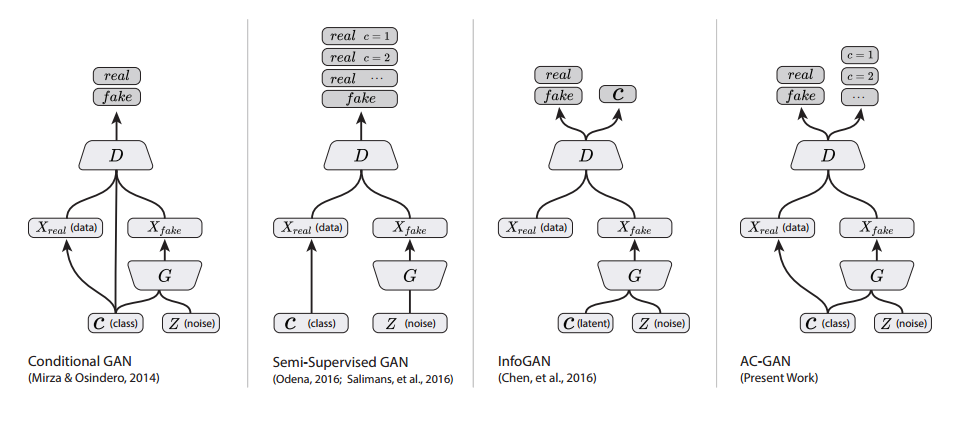
\includegraphics[width=1\textwidth]{images/class_conditional_gan.png}
    \caption{different architecture of variant of class conditioned GANs, in this project we implemented Conditioned GAN, infoGAN and AC-GAN. Class conditioned GANs have shown to improve the quality of generated output by explicitly providing the labels to model}
    \label{fig:mesh1}
\end{figure}
\medskip

\medskip



\begin{center}
    {\Large{\textbf{Style Translational GANs}}}
\end{center}
In cross domain image transfer tasks , we want to take an image from an input domain  Di  and then transform it into an image of target domain  Dt without necessarily having a one-to-one mapping between images from input to target domain in the training set.
\begin{itemize}
    \item Relaxation of having one-to-one mapping makes this formulation quite powerful - the same method could be used to tackle a variety of problems by varying the input-output domain pairs - performing artistic style transfer, adding bokeh effect to phone camera photos, creating outline maps from satellite images or convert horses to zebras and vice versa!! 
    \item Style Translation tasks are broadly performed by three GAN models - CycleGAN, DiscoGAN, and StarGAN.
    \item In a nutshell, CycleGAN works by taking an input image from domain  DA  which is fed to our first generator  GeneratorA→B  whose job is to transform a given image from domain  DA  to an image in target domain  DB . This new generated image is then fed to another generator  GeneratorB→A  which converts it back into an image,  CyclicA , from our original domain  DA  (think of autoencoders, except that our latent space is  Dt )
    \item CycleGAN and DiscoGAN use almost the same concept , losses and metrics but their they differ in their model structure . CycleGAN uses deep Residual connections whereas Model architecture of DiscoGAN is much simple and is very similar to DCGan . 
    \item CycleGan and DiscoGan and other style translation approaches approaches had limited scalability and robustness in handling more than two domains, since different models should be built independently for every pair of image domains. To address this limitation, StarGAN, a novel and scalable approach was made which can perform image-to-image translations for multiple domains using only a single model. Such a unified model architecture of StarGAN allows simultaneous training of multiple datasets with different domains within a single network. This led to StarGAN’s superior quality of translated images compared to existing models as well as the novel capability of flexibly translating an input image to any desired target domain.
\end{itemize}

\begin{figure}[h]
    \centering
    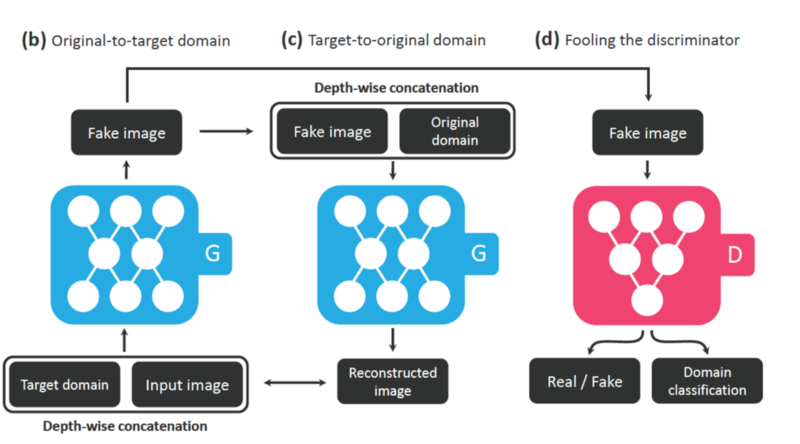
\includegraphics[width=0.7\textwidth]{images/style_stargan.png}
    \caption{Overview of StarGAN, consisting of two modules, a discriminator D and a generator G. (a) D learns to distinguish between
real and fake images and classify the real images to its corresponding domain. (b) G takes in as input both the image and target domain
label and generates an fake image. The target domain label is spatially replicated and concatenated with the input image. (c) G tries to
reconstruct the original image from the fake image given the original domain label. (d) G tries to generate images indistinguishable from
real images and classifiable as target domain by D.}
    \label{fig:mesh1}
\end{figure}
\medskip



\medskip
\begin{center}
    {\Large{\textbf{Special GANs}}}
\end{center}

Super-resolution GANs applies a deep network in combination with an adversary network to produce higher resolution images. As shown above, SRGAN is more appealing to a human with more details compared with the similar design without GAN (SRResNet). During the training, A high-resolution image (HR) is downsampled to a low-resolution image (LR). A GAN generator up-samples LR images to super-resolution images (SR). We use a discriminator to distinguish the HR images and back-propagate the GAN loss to train the discriminator and the generator (Figure 7).

\begin{figure}[h]
    \centering
    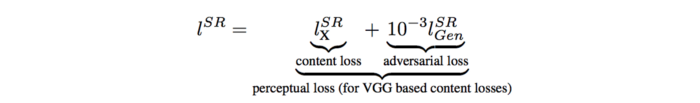
\includegraphics[width=.6\textwidth]{images/special_srganloss.png}
    \caption{perceptual loss which is used as metrics for optimmizing generator consist of weighted sum of content loss and adversial loss. Content loss ensure that the composition of output images and input images matches while adversial loss build up texture in super-resolution which other state-of-art SR model fail to generate}
    \label{fig:mesh1}
\end{figure}

\begin{figure}[h]
    \centering
    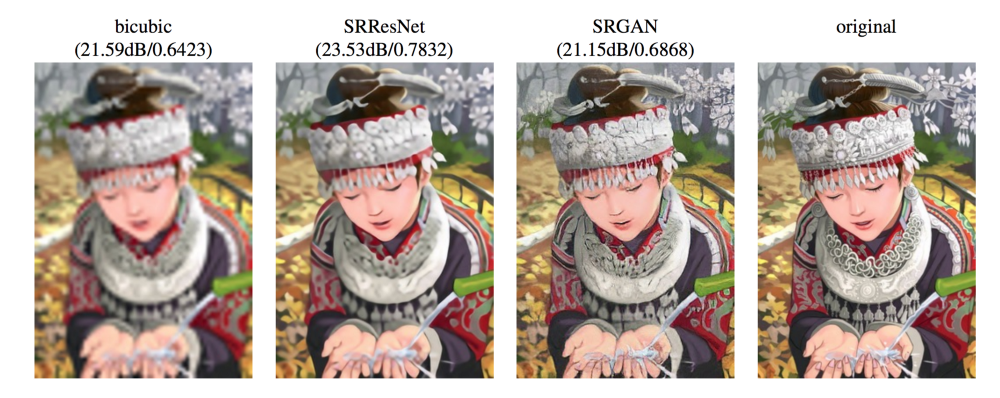
\includegraphics[width=1\textwidth]{images/special_srgan.png}
    \caption{From left to right: bicubic interpolation, deep residual network optimized for MSE, deep residual generative adversarial network optimized for a loss more sensitive to human perception, original HR image. Corresponding PSNR and SSIM are shown in brackets. [4× upscaling]}
    \label{fig:mesh1}
\end{figure}

\medskip
\begin{center}
    {\Large{\textbf{Techniques to Stabilize the Training of GANs}}}
\end{center}

CGANs could easily generate images with a simpler geometry like Ocean, Sky etc. but failed on images with some specific geometry like dogs, horses and many more. The CGAN was able to generate the texture of furs of dog but was unable to generate distinct legs.

This problem is arising because the convolution is a local operation whose receptive field depends on the spatial size of the kernel. Making the spatial size bigger so that it captures more of the image would decrease computational efficiency achieved by smaller filters and make the operation slow. Hence the author of SAGAN introduced a self-attention module (Figure 9) into convolutional GANs which  exhibits a better balance between the ability to model long-range dependencies and the computational and statistical efficiency. 


\begin{figure}[h]
    \centering
    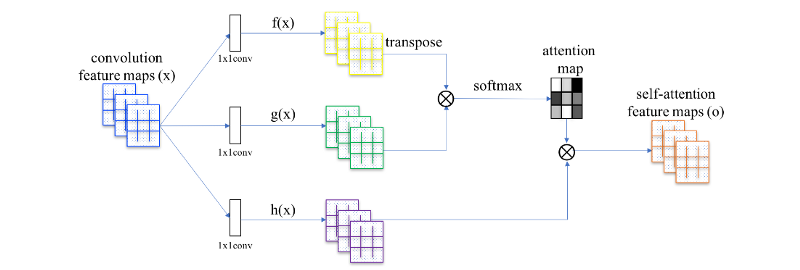
\includegraphics[width=.7\textwidth]{images/stablize_sa.png}
    \caption{The proposed self-attention module for the SAGAN. The \optimes denotes matrix multiplication. The softmax operation is performed on each row.}
    \label{fig:mesh1}
\end{figure}


Few Details from the paper (Summarized from the figure 10):
\begin{itemize}
    \item They used this self-attention layer in both the generator and discriminator
    \item They applied spectral normalization to the weights in both generator and discriminator, unlike the previous paper which only normalizes the discriminator weights. They set the spectral norm to 1 to constrain the Lipschitz constant of the weights. It’s just used for controlling the gradients. This spectral normalization idea was first introduced by Miyato et. al.
    \item They used a two-timescale update rule (TTUR) which is simply using different learning rate for both discriminator and generator.
    \item The metrics used in the paper are Inception Score (IS, higher is better) and Frechet-Inception Distance (FID, lower is better).
\end{itemize}

The paper explains with experiments how the Spectral Normalization and TTUR have helped the GAN to converge better. A picture of the same is shown below.
\medskip


\begin{figure}[h]
    \centering
    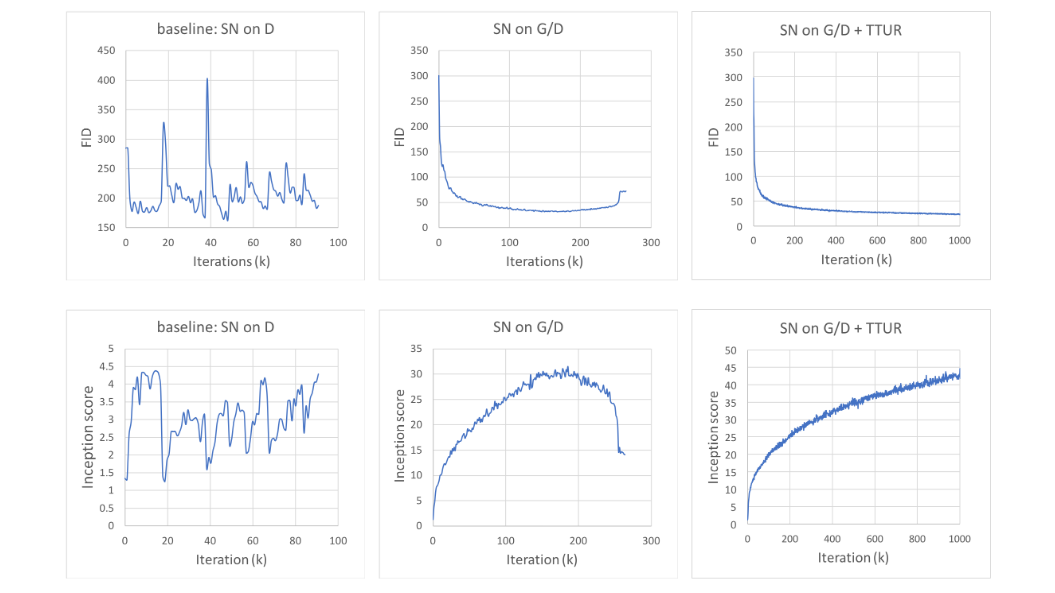
\includegraphics[width=1\textwidth]{images/stablize_summary.png}
    \caption{Training curves for the baseline model and our models with the proposed stabilization techniques, “SN on G/D” and two-timescale learning rates (TTUR). All models are trained with 1:1 balanced updates for G and D.}
    \label{fig:mesh1}
\end{figure}


\begin{center}
    {\Large{\textbf{NLP Gans}}}
\end{center}
\begin{itemize}
    \item GANs work by training a generator network that outputs synthetic data, then running a discriminator network on the synthetic data. The gradient of the output of the discriminator network with respect to the synthetic data tells you how to slightly change the synthetic data to make it more realistic.
    \item You can make slight changes to the synthetic data only if it is based on continuous numbers. If it is based on discrete numbers, there is no way to make a slight change.
    \item For example, if you output an image with a pixel value of 1.0, you can change that pixel value to 1.0001 on the next step. 
If you output the word "penguin", you can't change that to "penguin + .001" on the next step, because there is no such word as "penguin + .001". You have to go all the way from "penguin" to "ostrich".
    \item Since all NLP is based on discrete values like words, characters, or bytes, no one really knows how to apply GANs to NLP yet. 
    \item In principle, you could use the REINFORCE algorithm, but REINFORCE doesn't work very well, and no one has made the effort to try it yet as far as I know.
    \itemI see other people have said that GANs don't work for RNNs. As far as I know, that's wrong; in theory, there's no reason GANs should have trouble with RNN generators or discriminators. But no one with serious neural net credentials has really tried it yet either, so maybe there is some obstacle that comes up in practice.

\end{itemize}

% % % % % % % % % % %% % % % % % % % % % % % % % % % % % % % % % % % % % % % % % % % % % % % % % % % % % % 

\end{document}


